%************************************************
\chapter{Shaping the response in watersheds using a sensor network}\label{ch:shaping}
%************************************************
\vspace{1cm}

\section{Introduction}


Burdened by aging infrastructure, growing populations and changing hydrologic conditions, many municipalities struggle to adequately manage stormwater~\cite{Kerkez2016SmarterSystems}.
Flash flooding can occur when stormwater infrastructure is unable to convey runoff away from developed areas~\cite{Wright_2017}.
At the same time, pollutants from urban runoff---such as nutrients, heavy metals and microbes---can contaminate downstream waterbodies, damaging aquatic habitats and resulting in toxic algal blooms~\cite{Kerkez2016SmarterSystems}. Traditionally, civil engineers have addressed these challenges by building larger storage and conveyance infrastructure (e.g.\ basins and pipes). However, this approach suffers from a number of important disadvantages. First, new construction is expensive, and is often unfeasible for chronically underfunded stormwater departments~\cite{Montestruque_2015}. Second, static designs are inflexible to future changes in weather, population growth, and regulatory requirements~\cite{Wright_2017}. Third, overdesigned conveyance systems can cause flooding, erosion and damage to downstream property and ecosystems, which ultimately necessitates further remediation and construction~\cite{Kerkez2016SmarterSystems}. In the face of increasing urbanization and more frequent extreme weather events~\cite{Bronstert_2002, stocker_2014}, new strategies are needed to ensure effective management of stormwater.

\

In contrast to traditional \textit{steel-and-concrete} solutions, real-time control has emerged as a novel means to improve the performance of stormwater systems at minimal expense. Drawing on wireless communications, low-power microcontrollers, and modern advances in control theory, these systems achieve performance benefits by reconfiguring water infrastructure in real time~\cite{Bartos_2018, Kerkez2016SmarterSystems}. Real-time control of stormwater basins, for instance, can improve water quality following a storm event by enhancing removal of contaminants~\cite{Kerkez2016SmarterSystems}. Similarly, active regulation of discharges through constructed wetlands can improve water quality and rehabilitate aquatic habitats~\cite{Mullapudi2017, Bartos_2018}. More broadly, by controlling flows over a large network, operators can harness the latent treatment capacity of many distributed stormwater assets, effectively turning urban watersheds into distributed wastewater treatment plants~\cite{Bartos_2018, Kerkez2016SmarterSystems}.

\

A small number of studies have evaluated the benefits of real-time stormwater control. Most of these studies describe retrofits of isolated sites for rainwater capture and on-site pollutant treatment. Middleton and Barrett (2008) show that equipping existing retention basins with real-time controllers can reduce stormwater pollutant loads downstream by increasing the retention time of captured stormwater~\cite{Middleton_2008}. Roman et al. (2017) describe an adaptively-controlled rainwater harvesting system in New York City that captures 35--60\% more rainwater than conventional systems~\cite{Roman_2017}. Similarly, Klenzendorf et al. (2015) describe a rainwater harvesting pilot project and a retention basin retrofitted for real-time control in Austin, Texas~\cite{Klenzendorf_2015}. The authors show that the controlled retention basin reduces deposition of nitrogen and total suspended solids (TSS) into the downstream system. These studies demonstrate that active control can significantly improve the performance of existing sites at a lower cost than new construction. However, benefits are only examined at a local scale. This distinction is important, given that localized practices do not necessarily achieve the best system-scale outcomes. Indeed, some research indicates that when local best management practices are implemented without accounting for global outcomes, they can produce adverse flow conditions at the watershed scale~\cite{Emerson2005Watershed-ScaleBasins}.
%, their local benefits can quickly be masked by adverse global outcomes at the watershed scale

%\textcolor{blue}{However, since most optimization is carried out locally, relatively few studies have examined the potential of real-time control to downstream systems. This includes the ability to "shape" flows far downstream of the site being controlled, as coordinating between multiple sites to achieve improved performance throughout a larger service area.}

\

Currently, the benefits of coordinated stormwater control are poorly understood. Inspiration for the benefits of system-level control can be taken from sewer operations. While most sewer systems still only rely on local control logic, such as water level setpoints~\cite{Schutze2004RealToday}, recent work has demonstrated how wider benefits can be achieved through the cooperative action of multiple controllers working in tandem. The cities of Copenhagen and Barcelona, for instance, implement a combination of local rule-based control, and some higher-level optimization that jointly coordinates actions between groups of actuators~\cite{Mollerup2016}. Montestruque and Lemmon (2015) describe CSOnet, a sewer control network consisting of 120 sensors and 12 actuators in the city of South Bend, Indiana~\cite{Montestruque_2015}. This network uses dynamic control algorithms to adaptively balance hydraulic loads throughout the sewer’s interceptor lines, ultimately reducing combined sewer overflows (CSOs) by as much as 25\%. While these systems achieve impressive system-scale control of a large sewer networks, it is still unclear how lessons learned from these proprietary sewer control approaches may translate to the broader control of urban watersheds and separated stormwater systems. 

\

In this study, we describe an approach for
%characterizing control actions and
managing stormwater discharges across an urban watershed using internet-connected valves and sensors.
%The study relies on a new data set that has been collected by a large sensor and control network.
We show that by actively coordinating releases from two parallel retention basins, we can produce desirable flow regimes at a target location downstream, which would not be possible with passive infrastructure alone.
This study takes place in four phases.
%In the first phase, we leverage a network of sensors and controllers in the city of Ann Arbor, Michigan, which uses the \texttt{open storm} hardware and software stack \cite{Bartos_2018}.
%Using this existing wireless sensing and real-time control testbed,
In the first phase, we describe the development of a real-time stormwater control system in the city of Ann Arbor, Michigan. Building on an existing wireless sensing and control network described in Bartos et al. (2018)~\cite{Bartos_2018}, we demonstrate how static retention basins can be retrofitted with internet-controlled valves, and present a new method for controlling these basins using a controller scheduling application. In the second phase, we characterize the ability of the control network to shape the downstream hydrograph by releasing impulses of different sizes from two retention basins and determining the magnitude, travel time, and decay envelope of the resulting waves.  In the third phase, we use the data gathered from this exploratory analysis to determine the control input needed to produce a flat hydrograph at the outlet of the watershed. We discuss how this control strategy can be used to prevent erosion and reduce phosphorus loads into downstream waterbodies.
%facilitate contaminant uptake in a downstream constructed wetland.
Finally, in the fourth phase, we show how control inputs can be timed to produce synchronized and de-synchronized pulses at a downstream target location. In addition to demonstrating the precision of the control system, this experiment shows how interleaving pulses can be used to free up capacity in upstream retention basins without inducing synchronized flashy flows downstream. We discuss how these simple control ``building blocks'' can be used by system operators to achieve more sophisticated stormwater management targets. Unlike most existing systems, our control network uses an open-source hardware and software stack, making it freely available to municipalities that are interested in implementing their own smart stormwater control systems. Thus, when combined with supplementary \textit{how-to} documentation on \texttt{open-storm.org}, this study provides
%the beginnings
the foundation for an ``operator's manual'' for real-time control of urban watersheds.
%As such, this chapter not only provides experimental results, but it is also accompanied by significant supplementary "how-to" documentation on Open-Storm.org.

\section{Study area and technologies}

\begin{figure}
\centering
\includegraphics[width=\textwidth]{gfx/Chapter-2/fig_1_v2.png}
\caption{Overview of the study area. The map (left) shows the location of relevant control and sensor sites, additional sensor sites (light grey), flow paths between each site (dark grey), and the contributing area of the watershed (light blue). Site images (right) show the two control sites (A \& B) along with two downstream sensor locations (C \& D).
%For each control site, the control structure is shown, along with a detail photo of the valve apparatus.
}\label{fig-ch2:fig1}
\end{figure}
%\textcolor{blue}{Add volumes for each control site. (Ellsworth 19M Liters, CFP 7.5M L)PiP, Add legend (1) sensor nodes (squares) not used in study (grayed out) sensor nodes used (color code by site based on figures below) (2) control sites (circles, color coded); add upstream of Ellsworth. Note: Figure 3 now has CPF as Cite (C), so let's go with that. Control sites are (A) and (B)}

\subsection{Study area}

This study focuses on a wireless control network in the Mallets creek watershed---an urbanized creekshed located in the city of Ann Arbor, Michigan. This creekshed has been the focus of ongoing efforts to reduce peak flows and improve water quality~\cite{HRWC_2011}.
%(42.245529, -83.708835)
%[xx https://www.hrwc.org/wp-content/uploads/2012/08/HuronRiverReportFall2012.pdf xx]
The creekshed has an area of about 26.7 km$^2$ and contains streams that altogether exceed 16 km in length. These streams drain into the Huron River and ultimately the Great Lakes. With high areas of development and over 33\% imperviousness, little natural land is available for infiltration and uptake, resulting in flashy flows that erode stream banks and result in unstable habitats.
%On a normalized scale of 0 to 1 on the Richards-Baker flashiness index ~\cite{baker2004new}, the average flashiness of the creek (0.723) indicates that flows are significantly more flashy than the median flashiness of similarly sized streams throughout the state (0.314). 
These rapid flows drive stream erosion and increased transport of sediments and nutrients out of the watershed~\cite{HRWC_2011}. 
%[xx https://www.hrwc.org/wp-content/uploads/2011/11/MallettsCreek_BiotaTMDL_FINAL.pdf xx]
%At approximately 3.7 m/km, the average slope of the streams in the creekshed also exceeds the state average of 3.0 m/km, further contributing to flashy flows.
While there are no lakes in the creekshed, there are several natural and manmade stormwater basins that that have been constructed to help stabilize flows throughout the creekshed and mitigate the impacts of non-point source runoff.

\

To investigate the effects of real-time control on the creekshed, we deploy a control network that measures and regulates flows from two large stormwater basins. The control network consists of four sites centered around the main stem of the creek. Figure~\ref{fig-ch2:fig1} shows the locations of each of these four sites in the control network. Water first flows into a large retention basin with a storage capacity of 19M liters (site A), located at the most upstream point in the control network. From this retention basin, water travels 1.4 km downstream to a constructed wetland (site C), designed to slow the flow of water and remove contaminants. After passing through the wetland, water travels another 3 km until it is joined by flows arriving from a smaller retention basin with a storage capacity of 7.5M liters (site B). The combined flows exit the creek at the outlet of Mallet's creek (site D), after which they enter the Huron River. Internet-controlled valves are deployed at the two stormwater basins at sites A and B. These valves are used in subsequent experiments to regulate flows at the outlet of the creek.

\subsection{Technologies and Architecture}

Flows throughout the creekshed are measured and controlled using a custom wireless sensing and control network. This network is built using the \texttt{open storm} hardware and software stack, which has been described and documented in Bartos et al. (2018)~\cite{Bartos_2018}. The hardware layer uses an ultra-low power ARM Cortex-M3 microcontroller (Cypress PSoC), which implements the sensing and control logic in its firmware. Internet connectivity is achieved using a CDMA cellular modem (Telit DE910), which facilitates wireless bi-directional communication between the field device and a remote server. The full unit is powered using a solar-rechargeable 3.7V lithium-ion battery. To measure the hydrologic response of the system, wireless sensor nodes are deployed along the main stem of the creek. Each sensor node is equipped with an ultrasonic depth sensor (Maxbotix MB7384) to measure water levels (shown in Figure~\ref{fig-ch2:fig1}, Site C). At the time of writing, sensor nodes can be constructed using less than \$500 USD of parts. %, which include industrial-grade components and enclosures.
%While beyond the scope of this study, the platform also interfaces with a number of additional analog and digital sensors that can enable sensing of water quality, soil moisture, precipitation, and other hydrologically-relevant parameters. 

\

To control discharges throughout the creekshed, stormwater basins are retrofitted with one of two valves: (i) a 0.3 m diameter butterfly valve (Dynaquip MA44) (Figure~\ref{fig-ch2:fig1}, Site B) or (ii) a 0.3 m gate valve (Valterra 6912) mated to a linear actuator (AEI 6112CH) (Figure~\ref{fig-ch2:fig1}, Site A). Each control valve is connected to a sensor node. The valves are actuated by the microcontroller and powered by rechargeable 12V sealed lead-acid batteries. Solar panels allow the control sites to operate without line power. Assuming that the valve can be attached to a basin's outlet without structural modification, each control site can be constructed using less than \$3500 USD of parts at the time of writing.

%%%%%%%%%%%%%%%%
%The logic executed on each sensor and control node in the network is based on a \textit{polling} scheme (Figure 2).
\

Remote control of valves and sensors is implemented using a \textit{polling} scheme, in which field-deployed nodes request commands from a remote server (Figure~\ref{fig-ch2:fig2}). To conserve power, nodes spend most of their time in a deep sleep state, consuming only 1--10 $\mu$A of current. Upon waking up, each node takes sensor readings and transmits the readings to a cloud-hosted time series database (InfluxDB) via authenticated (and optionally encrypted) \textit{HTTP} requests. Before going back to sleep, the node polls a set of commands from a dedicated feed in the same database. The commands may include, but are not limited to, changing the sampling frequency, triggering additional sensor readings, or opening a valve.
%In this fashion, the node does not accept, nor require, any direct incoming communications, but instead only follows commands from an authenticated central server.
Operations can be cancelled and rescheduled either by the application or by an operator. This is useful if, for example, the application detects that a control action was not successfully executed and that pending operations need to be rescheduled. Most importantly, the database supports modern web service standards and application programming interfaces (APIs), which allow the control logic to be quickly implemented via simple web applications. These applications can be written in any number of popular programming languages (Python, Matlab, etc). This feature improves flexibility, reduces reliance on low-level firmware updates, and allows for the seamless integration of external data sources, such as public weather forecasts~\cite{Wong_2016b, Bartos_2018}.
%%Real-time environmental sensor data: An application to water quality using web services

\

For the experiments described in this study, field devices in the creekshed are controlled using a simple Python web application. This application can be executed in either automatic or manual mode. In automatic mode, the application queries water level sensor feeds, rainfall forecasts, and external flow measurements from a publicly-listed measurement station at the outlet of the creekshed (\href{https://waterdata.usgs.gov/usa/nwis/uv?04174518}{USGS 04174518}). Based on these sensor readings, new commands are then written to the database to open and close valves. In manual operation, a predefined set of commands is written to the database, then subsequently executed by the field device. For this study, the manual operation mode is used. 
%An acknowledgment scheme is implemented, wherein field devices write flags to the database once a command is successfully executed. This allows the operator to determine when commands have been successfully executed, and also prevents commands from being executed multiple times.
The application toolchain is implemented on an Amazon Web Services (AWS) medium-sized linux Elastic Compute Cloud (EC2) instance. 


%%In this study, sensor data is used to characterize the travel times from each control point to the outlet of the creekshed. As well as logging sensor data, future commands can be queued manually by an operator or automatically by a script, meaning sensor nodes and valves can be asleep and execute the commands upon waking up. This functionality provides the foundation for coordinated flow control throughout the creekshed.

%With the ability to automatically monitor and control flows throughout the creekshed,
%The process for designing new flow experiments was streamlined to updating an app.
%Control experiments are executed using a custom-built app, which schedules releases from each of the two retention basins. This app is implemented in Python, but could also be done in other languages such as Matlab. The app schedules times to open and close each each valve by submitting \texttt{HTTP} requests with the appropriate credentials to a web platform (Figure 2). Upon waking up, each valve is programmed to query the platform for its next scheduled control action, which it then executes. Upon executing the control action, the sensor node updates its status on the platform before returning to sleep mode. 

\begin{figure}
\centering
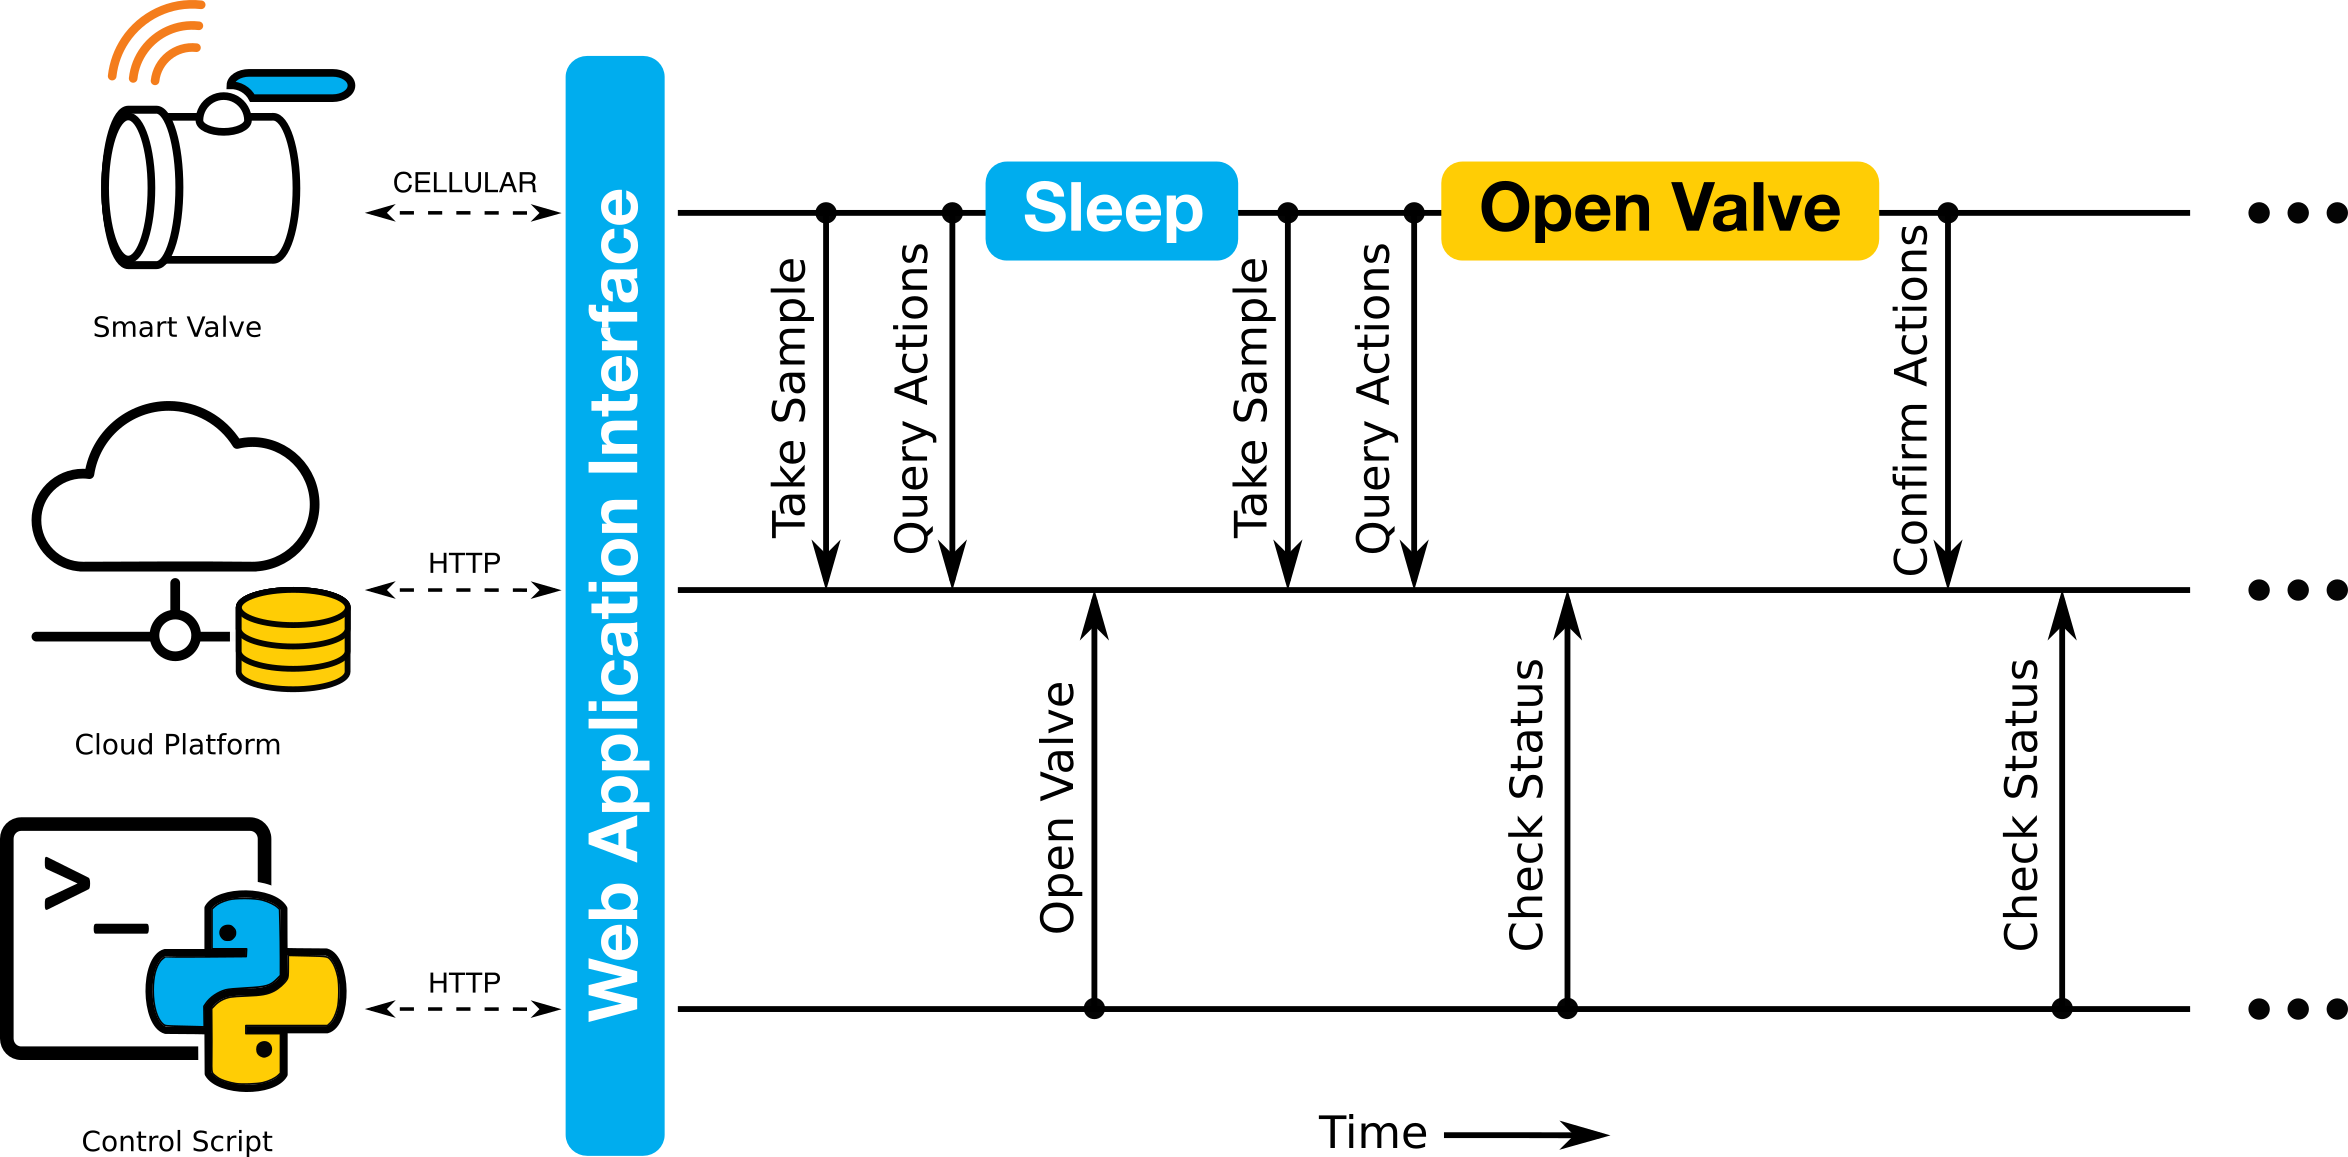
\includegraphics[width=\textwidth]{gfx/Chapter-2/Figure_2_Control_Flow_Landscape.png}
\caption{Control system architecture. %Each control node spends the vast majority of time in a deep sleep state, conserving battery resources.
Field-deployed nodes use a polling system to download and execute commands issued from a remote server.
Control actions can be specified manually, or through automated web applications and scripts.
%Nodes spend the majority of time in sleep mode to conserve battery. Upon waking up, nodes report the most recent sensor readings and query pending commands from a central database. %Commands can be entered manually into the databse, but are most open written by dedicated web applications, such as \texttt{Python} scripts.
%Commands can be written to the database manually, or automatically, using dedicated web applications and scripts.
}\label{fig-ch2:fig2}
\end{figure}

\section{Characterizing control actions}
%(Fig 3ab, Fig 4, Fig 5)

Before evaluating potential control strategies, we first characterize the ability of each control site to shape downstream flows. Specifically, we quantify the travel time $P$ and decay time $D$, of various waves as they move between the originating control site and the outlet of the watershed. The characterization is accomplished by releasing pulses of different durations 
%and magnitudes 
from each stormwater basin and then observing the resulting waves that these pulses generate downstream. To limit confounding effects caused by rainfall, these experiments are carried out during dry conditions (at least 4 days following a storm). Figure~\ref{fig-ch2:3} shows a 1-hour release, 4-hour release, and 48-hour release from retention basin A (shown left to right, respectively). The 48-hour release empties the retention basin, meaning that this release characterizes the maximum possible output from site A. The travel times for each wave from site A to site C are approximately 3.5 hours (time to start of rise) and 6--8 hours (time to peak), with faster rise times for the larger releases due to nonlinearities in the speed of wave propagation. The decay times for each release are 6 hours, 18 hours and 44 hours, respectively. From this experiment, it can be seen that the maximum change in flow that site A can generate at the outlet is roughly 0.17 m$^3$/s.
%Interestingly, the change in flow effected by a 48-hour release is almost the same as the change in flow resulting from a 4-hour release
Similar experiments are used to characterize site B. From these experiments, we estimate average travel times from site B to the outlet of 1.5 hours (time to start of rise) and 1.8 hours (time to peak), with an average decay time of 3 hours, and a maximum change in flow of approximately 0.2 m$^3$/s.

\begin{figure}
    \centering
    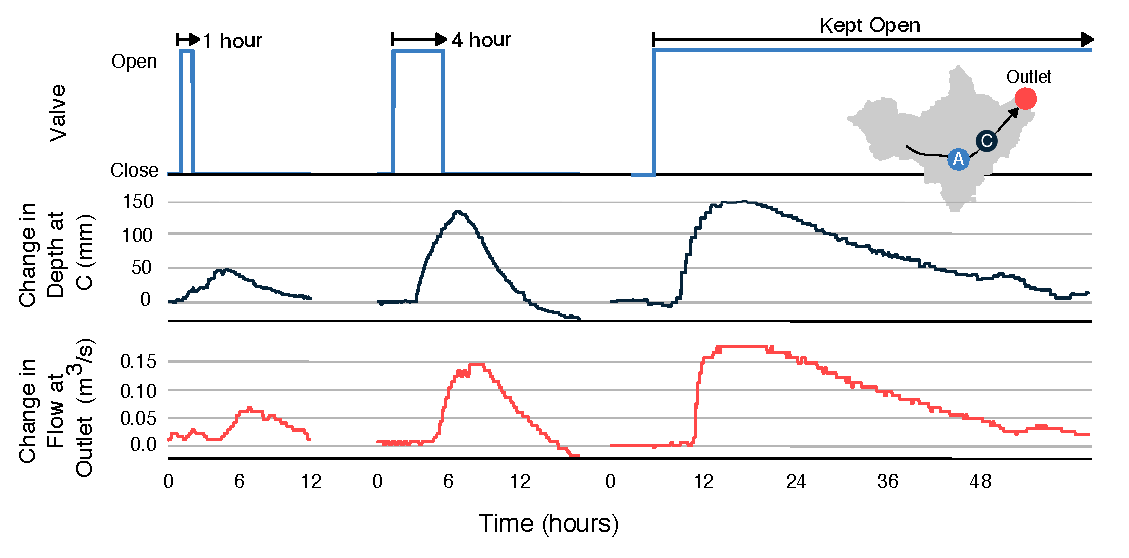
\includegraphics[width=\textwidth]{gfx/Chapter-2/fod.eps}
    \caption{Characterization of
    %the response of 
    control actions from site A. In the first two experiments,
    the valve at site A is opened for 1-hour and 4-hour durations. For the third experiment, the valve is held open indefinitely.
    %as well as opened without being closed. The
    %flows
    The resulting waves travel through
    %a midway point
    a constructed wetland (site C) %, black line)
    before arriving at the outlet of the watershed. Wave depth (black line) is measured at the wetland, while flow rate (red line) is measured at the outlet.}\label{fig-ch2:3}
\end{figure}

\

In addition to release duration, sites are also characterized with respect to the hydraulic head (water level) of the originating retention basin. Figure~\ref{fig-ch2:4} shows the result of releasing three 1-hour pulses from site B, without allowing the basin to refill between releases. While the same duration is used for each release, the hydraulic head (stored volume) of the retention basin decreases with each pulse. Thus, the resulting wave becomes smaller with each successive opening of the valve, even though the same input signal is used. In spite of this difference, the travel time and decay time of the wave remain consistent between each release.
%, with a time-to-peak of roughly 1.5 hours and a decay time of roughly \textcolor{blue}{3} hours.
The magnitude of the resulting wave varies from roughly 0.2 m$^3$/s to 0.13 m$^3$/s, depending on the water level in the basin. 

\begin{figure}
    \centering
    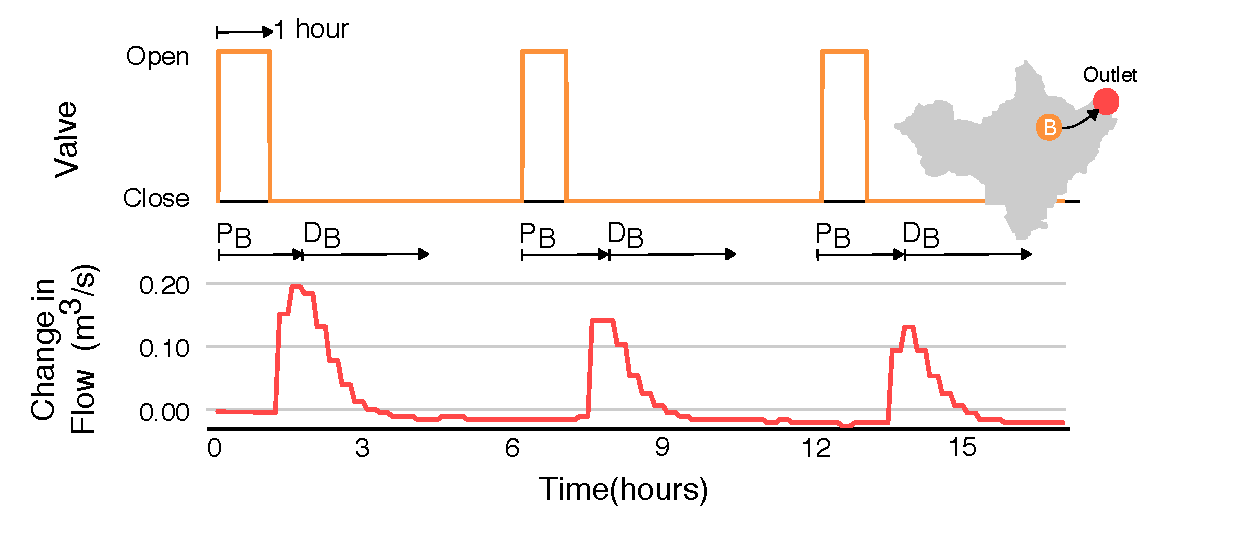
\includegraphics[width=\textwidth]{gfx/Chapter-2/Figure5_F.eps}
    \caption{Characterization of control actions originating from site B. Three subsequent pulses are released. While the duration of each control pulse is the same (1 hour), the magnitude of the flow
    %s decreases since less water is available in the basin each time.
    at the outlet decreases because the hydraulic head (pressure) in the basin is reduced with each release.
    }\label{fig-ch2:4}
\end{figure}

\

Although retention basin B is significantly smaller than retention basin A, it can produce a comparable change in flow at the watershed outlet (approximately 0.2 m$^3$/s). This effect can be attributed to two main factors. First, site B is located closer to the outlet (3.0 km as opposed to 5.9 km for site A), meaning that the wave is subject to less hydraulic dispersion. Second, the retention basin at site B is elevated higher above the receiving stream, meaning that flows exit the control structure more rapidly than flows released from site A. Thus, compared to site A, site B produces short pulses with a rapid onset and large peak. Despite its relatively smaller volume, control actions from site B must thus be tailored to avoid generating flashy flows at the outlet.
%\textcolor{blue}{If we annotate fig 1 with volumes and travel path lengths (maybe even elevation), then we could refer to this easily in this paragraph}

\

One crucial result of these experiments is that for the purposes of control, nonlinearities in wave propagation can be safely ignored. Shallow-water waves exhibit a nonlinear relationship between wave height and wave speed, meaning that larger waves propagate faster~\cite{kinnmark2012shallow}. %This nonlinear relationship is the reason why hydrographs are typically skewed to the left (given that the taller portions of the wave travel faster than the shorter portions).
If these nonlinearities were significant, then control strategies would need to account for changes in travel time due to (i) variations in release durations, (ii) variations in basin head, and (iii) superposition of waves originating from different locations.
For the system examined in this study, the effect of these nonlinearities is small. Namely, while nonlinearities in wave propagation affect the shape of the resulting hydrograph (skewing the peak toward the left), they do not significantly affect the bulk travel time of an isolated wave.
Specifically, the travel times for Site A and Site B remain consistent (3.5 hours and 1.5 hours, respectively) despite scheduling releases of different durations and magnitudes. This result is consistent with findings from previous studies that use linear dynamics for stormwater system control~\cite{Litrico_2004, Marinaki_2003, Garcia_2015}.
Thus, for the scale of our creekshed the travel time of a wave originating at an upstream stormwater basin can be considered independent of both the amount of water released and the water level of the originating basin. Moreover, superposition of two waves from two parallel sources does not effect a noticeable change in bulk wave speed. This result suggests that for the purposes of control, the channel network may be approximated as a linear system in which waves originating from each retention basin can be superimposed in order to produce a desired output hydrograph downstream. 

% No longer current?
%\textcolor{blue}{Given the distance between sites, control actions may not be detectable by downstream sensors due to dispersion or poor measurement accuracy. To quantify the smallest possible control action that could be detected downstream, each site was filled to capacity, after which the valve was opened for a short duration and then closed (starting at XX mins, with increments of YY mins). The smallest duration that resulted in a detectable change in downstream water levels was noted (example Figure 3a for site AA). The largest possible control actions was also quantified by filling a control site to capacity and keeping the valve opened until the entire site drained (example Figure 3b for site AA).}

\

By characterizing the downstream response to various impulsive inputs, these initial experiments yield a set of ``building blocks” that are subsequently used to achieve more complex control objectives at the watershed outlet.
%These building blocks---which are characterized by their magnitude, decay period, travel time---can be combined to generate more complex waveforms downstream.
While the propagation of waves within a channel network is described by nonlinear equations, we find that a linear system approximation adequately describes the dynamics needed to generate control strategies. %these approximations sufficiently describe unit impulses that could be sequenced and superimposed to create desired hydrograph shapes throughout the watershed.
Thus, the characterization experiments described in this section are conceptually analogous to quantifying the unit impulse response of a linear system. This framework suggests that desired waveforms can be generated via simple linear combinations of known input signals.
%which can then be used to produce control actions to create specific conditions or set points at the outlet of the watershed.
With this conceptual model in hand, we carry out a number of control experiments to showcase the utility of the stormwater control network. First, we show how pulse-width modulation of a valve can be used to produce a flat hydrograph that meets but does not exceed a given flow threshold. Next, we show how valve releases can be timed to generate synchronized and desynchronized waves at the outlet. These experiments provide recipes for managing releases from upstream retention basins while simultaneously fostering desirable flow conditions downstream.
%\textcolor{blue}{For example, the system could be pulsed in short bursts to create small, non-overlapping hydrographs at the outlet of the watershed (Figure 5). This experiment highlights the precision, consistency, and predictability that can be achieved by a single control site.}

\section{Set-point hydrographs}

Real-time control can be used to flatten downstream hydrographs, helping to reduce erosion and maintain healthy aquatic ecosystems. In passive stormwater systems, hydrographs often exhibit a distinct peak, preceded by a rapid rise and followed by a slower decay. While typically associated with rain events, this phenomenon can also be observed when water is released from a retention basin (see Figures~\ref{fig-ch2:3} and~\ref{fig-ch2:4}). Peak flows that exceed downstream capacity will often lead to flooding. Furthermore, urban streams can become unstable if a critical flow velocity or flow rate is reached~\citep{bledsoe2002stream}. Exceedance of these thresholds may lead to ecological damage and stream erosion, as well the mobilization of sediments. These sediments in turn may carry nutrients, metals and other pollutants downstream, impairing water quality and promoting the growth of algal blooms~\cite{Michalak2013Record-settingConditions}. This particular impairment underpins the major challenge of ``urban stream syndrome'', forcing many cities to spend millions of dollars to reduce downstream flow rates~\cite{schilling2008greening, wise2008green}. 
%\textcolor{red}{(xx cite
%[http://www.esf.edu/cue/documents/Greeningtherustbelt.pdf],
% Philadelphia's invested $16 million (p 456)
%[http://74.208.132.129/repository/APA-article.greeninfrastructure.080108.pdf]
% $285k per city block; Milwaukee invested $12 million; Portland invested $50 million over 5 yearsxx)}
While active control has been proposed as a means to condition stormwater flows, the specific control strategies needed to achieve stable flow conditions within an urban watershed are currently not well understood.

\

To address this challenge, a sequence of control actions is designed to yield a constant set-point condition at the outlet of the watershed. Specifically, we aim to create a flat hydrograph, for which the flow rate remains close to (but does not exceed) a specified value. While the set-point used in this experiment is chosen arbitrarily, this threshold may be chosen to control for objectives related to downstream flooding and water quality---for instance, ensuring that the critical flow threshold for sediment transport is not surpassed.
%To investigate the viability of such an approach, a low setpoint is chosen---corresponding to the peak of our ``building block” hydrograph \textcolor{red}{(XX m3/s, see Figure xx)}. 
To achieve a constant set-point flow rate, we derive inspiration from \textit{pulse-width modulation}---a method used in electrical systems to generate analog signals from discrete digital pulses. Isolated pulses of water are emitted from the control site, spaced apart such that the arrival time of each wave overlaps with the receding limb of the prior wave. As the pulses travel through the channel network, they disperse, causing the individual waves to overlap and combine. The resulting superposition of partly-dispersed waves results in an approximately constant flow rate.
%This result is particularly promising considering the low cost of our control system and the distance between control site and watershed outlet (5.9 km).
%While this control strategy is relatively simple and only dependent on timing information, if the \textcolor{blue}{watershed transfer were approximated as a low-pass filter the approach becomes analogous to pulse modulated control.}

\

\begin{figure}
    \centering
    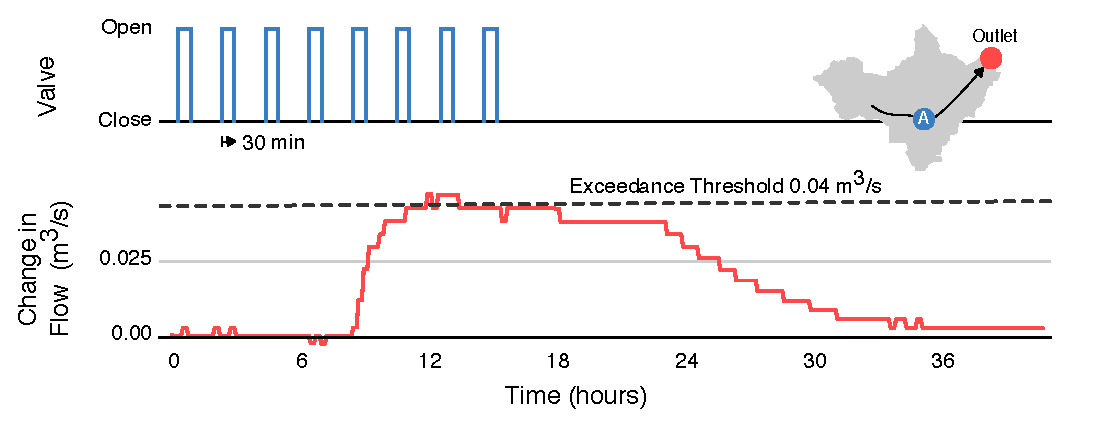
\includegraphics[width=\textwidth]{gfx/Chapter-2/Figure7.eps}
    \caption{Generating a set-point hydrograph. Small, evenly spaced pulses (30-minute duration) are released from the controlled basin. The pulses disperse as they travel through the 6 km-long stream, leading to a relatively flat response at the outlet of the watershed.}\label{fig-ch2:5}
\end{figure}

As seen in the hydrograph response (Figure~\ref{fig-ch2:5}), the ``flat hydrograph'' objective is achieved by modulating the valve position in successive 30-minute pulses. The flows at the outlet remain approximately flat, without significantly exceeding a setpoint of 0.04 m$^3$/s. Of course, the shape is not perfectly flat, given the large distance between the two sites and nonlinearities inherent in wave propagation. However, these experimental results show that active modulation of a valve can produce highly stable flow conditions downstream that would not be possible using passive infrastructure alone. In a real-world scenario, this control strategy could be used to drain a watershed as fast as possible without exceeding a critical flood conditions downstream. Minimizing the change in flows downstream also reduces the likelihood of stream erosion. From our prior studies in this creekshed that were not affected by real-time control~\cite{Wong_2016}, it can be estimated that pollutant concentrations during this flat stage were no greater than 127 mg/L for sediment and 0.209 mg/L for total phosphorus. For comparison, keeping the valve open would have resulted in concentrations of at least 390 mg/L for sediment and 0.618 mg/L for total phosphorus. By modulating the valve position to achieve a relatively flat and steady outflow, the control actions likely reduced the total mass of solids and phosphorus
%otherwise responsible for
that would otherwise contribute to ecological damage and harmful algal blooms. Future studies will confirm and refine these estimates by measuring real-time water quality changes that result from control.

%a peak increase in flow of 1.30 m$^3$/s corresponds to a peak sediment concentration of 776 mg/L and a peak total phosphorous concentration of 0.98 mg/L. By modulating the valve opening, the change in flows better approximates steady baseflow conditions, where average baseflow concentrations were no greater than 127 mg/L and 0.209 mg/L for sediment concentrations and total phosphorus, respectively, whereas during wet weather events, concentrations were as at least 390 mg/L for sediment concentrations and 0.618 mg/L for total phosphorus. By modulating the valve position to achieve a relatively flat and steady outflow, this reduced the total mass of solids and phosphorus otherwise responsible for ecological damage and harmful algal blooms.

\section{Coordinated releases between multiple control sites}

Motivated by the larger goal of watershed-scale control, a final experiment is devised to evaluate the level of precision that can be achieved when coordinating releases from multiple sites. Namely, we schedule releases from the two controlled basins in order to produce synchronized and interleaved pulses at the outlet. Before running the experiment, we first determine the control signals needed to generate the combined and interleaved waves, respectively, by assessing the travel time and decay time of waves released from each retention basin. Figure~\ref{fig-ch2:6} shows the hydrographs resulting from 1-hour pulses released simultaneously from site A and site B. Based on the travel times of each wave, it can be seen that in order to achieve a synchronized wave at the outlet, a 1-hour release from site B must be scheduled approximately six hours after a 1-hour release from site A. Conversely, to achieve an interleaved pattern at the outlet, the following pulse train can be used: (i) release a 1-hour pulse from site A, (ii) release a pulse from site B approximately 12 hours later, (iii) release a pulse from site A after waiting an additional four hours, and (iv) repeat the pattern starting at step (ii).

\

\begin{figure}
    \centering
    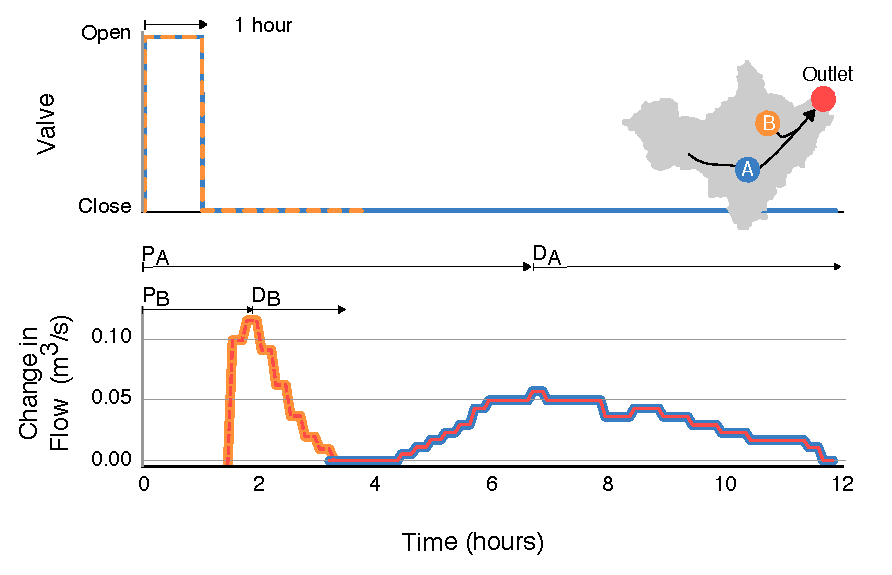
\includegraphics[width=\textwidth]{gfx/Chapter-2/Figure4.eps}
    \caption{Flows at outlet of watershed resulting from 1 hour releases from each control site. Time to peak $P$, magnitude, and decay time $D$ for each release are labeled.}\label{fig-ch2:6}
\end{figure}


Once the input signals required to produce each desired shape are known, we schedule a series of commands to be executed by each valve. The experiment is divided into two stages.
%, for which the known travel time was used to create two desired conditions: superimposed and interleaved waves.
During the first stage, flows from the control sites are released such that the peaks of the hydrographs overlap.
%, thus demonstrating the level of fine precision that can be achieved when matching specific features of individual hydrographs (Figure 6a). 
In the second stage of the experiment, the flows are released off-phase, such that the flows arriving from one site begin exactly when the flows from the other site recede.
%This demonstrates the tight level of tolerance that can be achieved when interleaving flows from individual sites.
Figure~\ref{fig-ch2:fig6} shows the result of this experiment, with the overlapping waves occurring from hours 6 to 15, and the interleaved waves occurring from hours 15 to 44. As hypothesized earlier, the superposition of waves is approximately linear. In other words, the maximum change in flow is approximately equal to the sum of the maximum flow of each component wave. Moreover, the superposition of the two waves does not appear to appreciably change the bulk travel time.

\

\begin{figure}
    \centering
    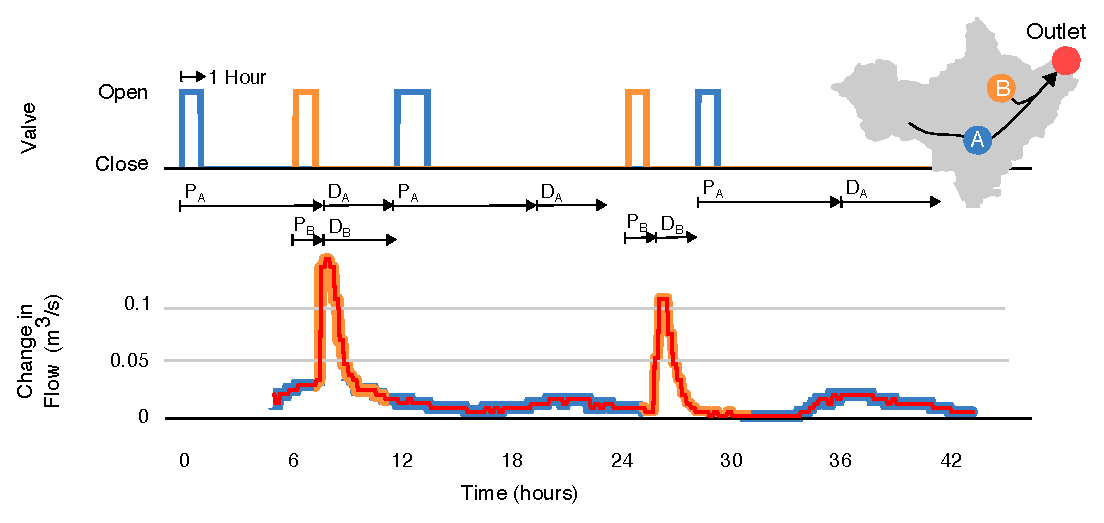
\includegraphics[width=\textwidth]{gfx/Chapter-2/Figure6.eps}
    \caption{Superposition and interleaving of waves from retention basins A and B.
    %The firf individual hydrographs, while the remaining control actions achieve interwoven, non-overlapping hydropgraphs.
    Overlapping waves (coincident peaks) are generated from hours 6 to 12. Interleaved waves (off-phase peaks) are generated from hours 18 to 44.
    }\label{fig-ch2:fig6}
\end{figure}

This experiment shows that real-time control of stormwater systems can achieve precise control over downstream flow conditions, and also suggests a strategy for coordinating releases in order to remove stormwater from retention basins while simultaneously achieving target flow conditions downstream. Like the set-point experiment, an interleaving control pattern can be used to de-water upstream retention basins without exceeding a particular flow threshold downstream. When waves generated by several upstream retention basins combine, they can generate large, flashy flows at a downstream location.
%Due to the nonlinear effects of wave propagation, these combined waves may be taller and travel faster than the component waves that comprise them.
This in turn can contribute to erosion of the surrounding channel. For this reason, it is desirable to avoid the collision of waves from two different upstream sources. By interleaving flows from upstream retention basins, one can free up capacity in the system without generating adverse flow conditions downstream. More broadly, the results of this experiment demonstrate the fine level of flow control that can be achieved across urban watersheds using a low-cost sensor and control network. While the underlying control logic only uses rudimentary time-of-travel metrics it nonetheless produces desirable flow regimes that would be difficult to achieve with passive infrastructure alone. As such, this experiment builds a foundation for more complex control strategies by verifying that the watershed responds consistently and predictably to individual control actions. This result suggests that future studies may one day demonstrate more complex, possibly near-arbitrary, hydrograph shapes. Time of travel may not be sufficient for such approaches, however, and more complex and analytical control techniques should be considered. 

\section{Conclusions}

This study shows how internet-connected stormwater control valves can be used to shape streamflows within a large urban watershed. To our knowledge, this study is the first to document how coordinated releases between multiple stormwater control sites can satisfy system-scale watershed performance goals---such as maintaining downstream flow at a constant rate or preventing sediment transport. Building on an existing wireless sensor network, we demonstrate how static stormwater retention basins can be retrofitted with internet-controlled valves to enable active control at a low cost. 
%A cloud-based scheduling application is then developed to enable remote execution of complex control actions.
%After building the control infrastructure,
% We then characterize the capabilities of the system by releasing various pulses from the upstream retention basins and subsequently measuring the downstream response.
%This characterization process yields the travel times, decay times, and magnitudes for releases of various sizes.
Characterizing the system in a series of exploratory experiments,
we find that a linear approximation is sufficient to describe the downstream response associated with a given input. Next, we use the system to generate two flow conditions downstream: (i) a set-point hydrograph in which flow is maintained at a roughly constant rate, and (ii) a series of overlapping and interleaved waves. We find that pulse-width modulation of upstream valves generates a flat downstream response. Similarly, interleaving of discharges provides an effective tool for emptying upstream retention basins without inducing flashy flows downstream. In addition to demonstrating the precision of the control system, these experiments suggest strategies for managing stormwater transfers across a watershed while maintaining desired flow conditions. To make the smart stormwater system described in this chapter accessible to water managers worldwide, all hardware, software and documentation for this project are made available at \texttt{open-storm.org}.
